\documentclass[12pt,a4paper]{report}
\usepackage[utf8]{inputenc}
\usepackage[french]{babel}
\usepackage[T1]{fontenc}
\usepackage{listings}
\usepackage{xcolor}
\usepackage{amsmath}
\usepackage{graphicx}
\usepackage{float}
\usepackage{hyperref}

% Configuration des listings pour le code Draw++
\lstdefinelanguage{Draw++}{
  keywords={var, const, if, else, elif, while, for, int, float, bool, string, color,
           cursor, window, true, false, BLACK, WHITE, RED, GREEN, BLUE},
  sensitive=true,
  comment=[l]{//},
  morecomment=[s]{/*}{*/},
  morestring=[b]",
  morestring=[b]'
}

\lstset{
  language=Draw++,
  basicstyle=\ttfamily\small,
  numbers=left,
  numberstyle=\tiny,
  numbersep=5pt,
  frame=single,
  breaklines=true,
  keywordstyle=\color{blue},
  commentstyle=\color{green!60!black},
  stringstyle=\color{red},
  showstringspaces=false
}
\lstdefinestyle{customStyle}{
    basicstyle=\footnotesize\ttfamily\color{black},
    keywordstyle=\color{black},
    stringstyle=\color{black},
    commentstyle=\color{black},
    literate={e}{{\'e}}1 {è}{{\`e}}1 {à}{{\`a}}1,
    frame=single,
    breaklines=true
}




\title{Rapport de Projet : Draw++}
\author{
    Chekhab Elias \\
    Guihot Nathan \\
    Aissaoui Ahmed \\
    Zheng Lise \\
    Benmansour Firas
}
\date{\today}

\begin{document}

\maketitle
\tableofcontents

\chapter{Introduction}
Draw++ est un langage de programmation specialement conçu pour la creation graphique, visant à simplifier l'interaction avec des elements visuels à travers un ensemble d'instructions simples et intuitives. Ce langage a ete conçu pour offrir une approche accessible et directe de la programmation graphique, permettant aux utilisateurs de dessiner des formes.\\

Le projet inclut non seulement le langage de programmation proprement dit, mais aussi un environnement de developpement integre (IDE) specialement conçu pour faciliter l'ecriture, le test, et le debogage du code. L'IDE permet aux utilisateurs de visualiser immediatement l'effet de leur code sur des graphiques à l'ecran, favorisant une approche interactive et reactive de la programmation. Grâce à des fonctionnalites telles que la coloration des erreurs syntaxiques, le debogage et la gestion des erreurs, l'IDE rend l'experience de programmation plus intuitive et accessible, même pour les debutants.

\chapter{La Syntaxe du Langage}

\section{Grammaire BNF du Langage Draw++}
Voici la grammaire formelle du langage Draw++ exprimee en notation BNF :
\begin{figure}[H]
    \centering
    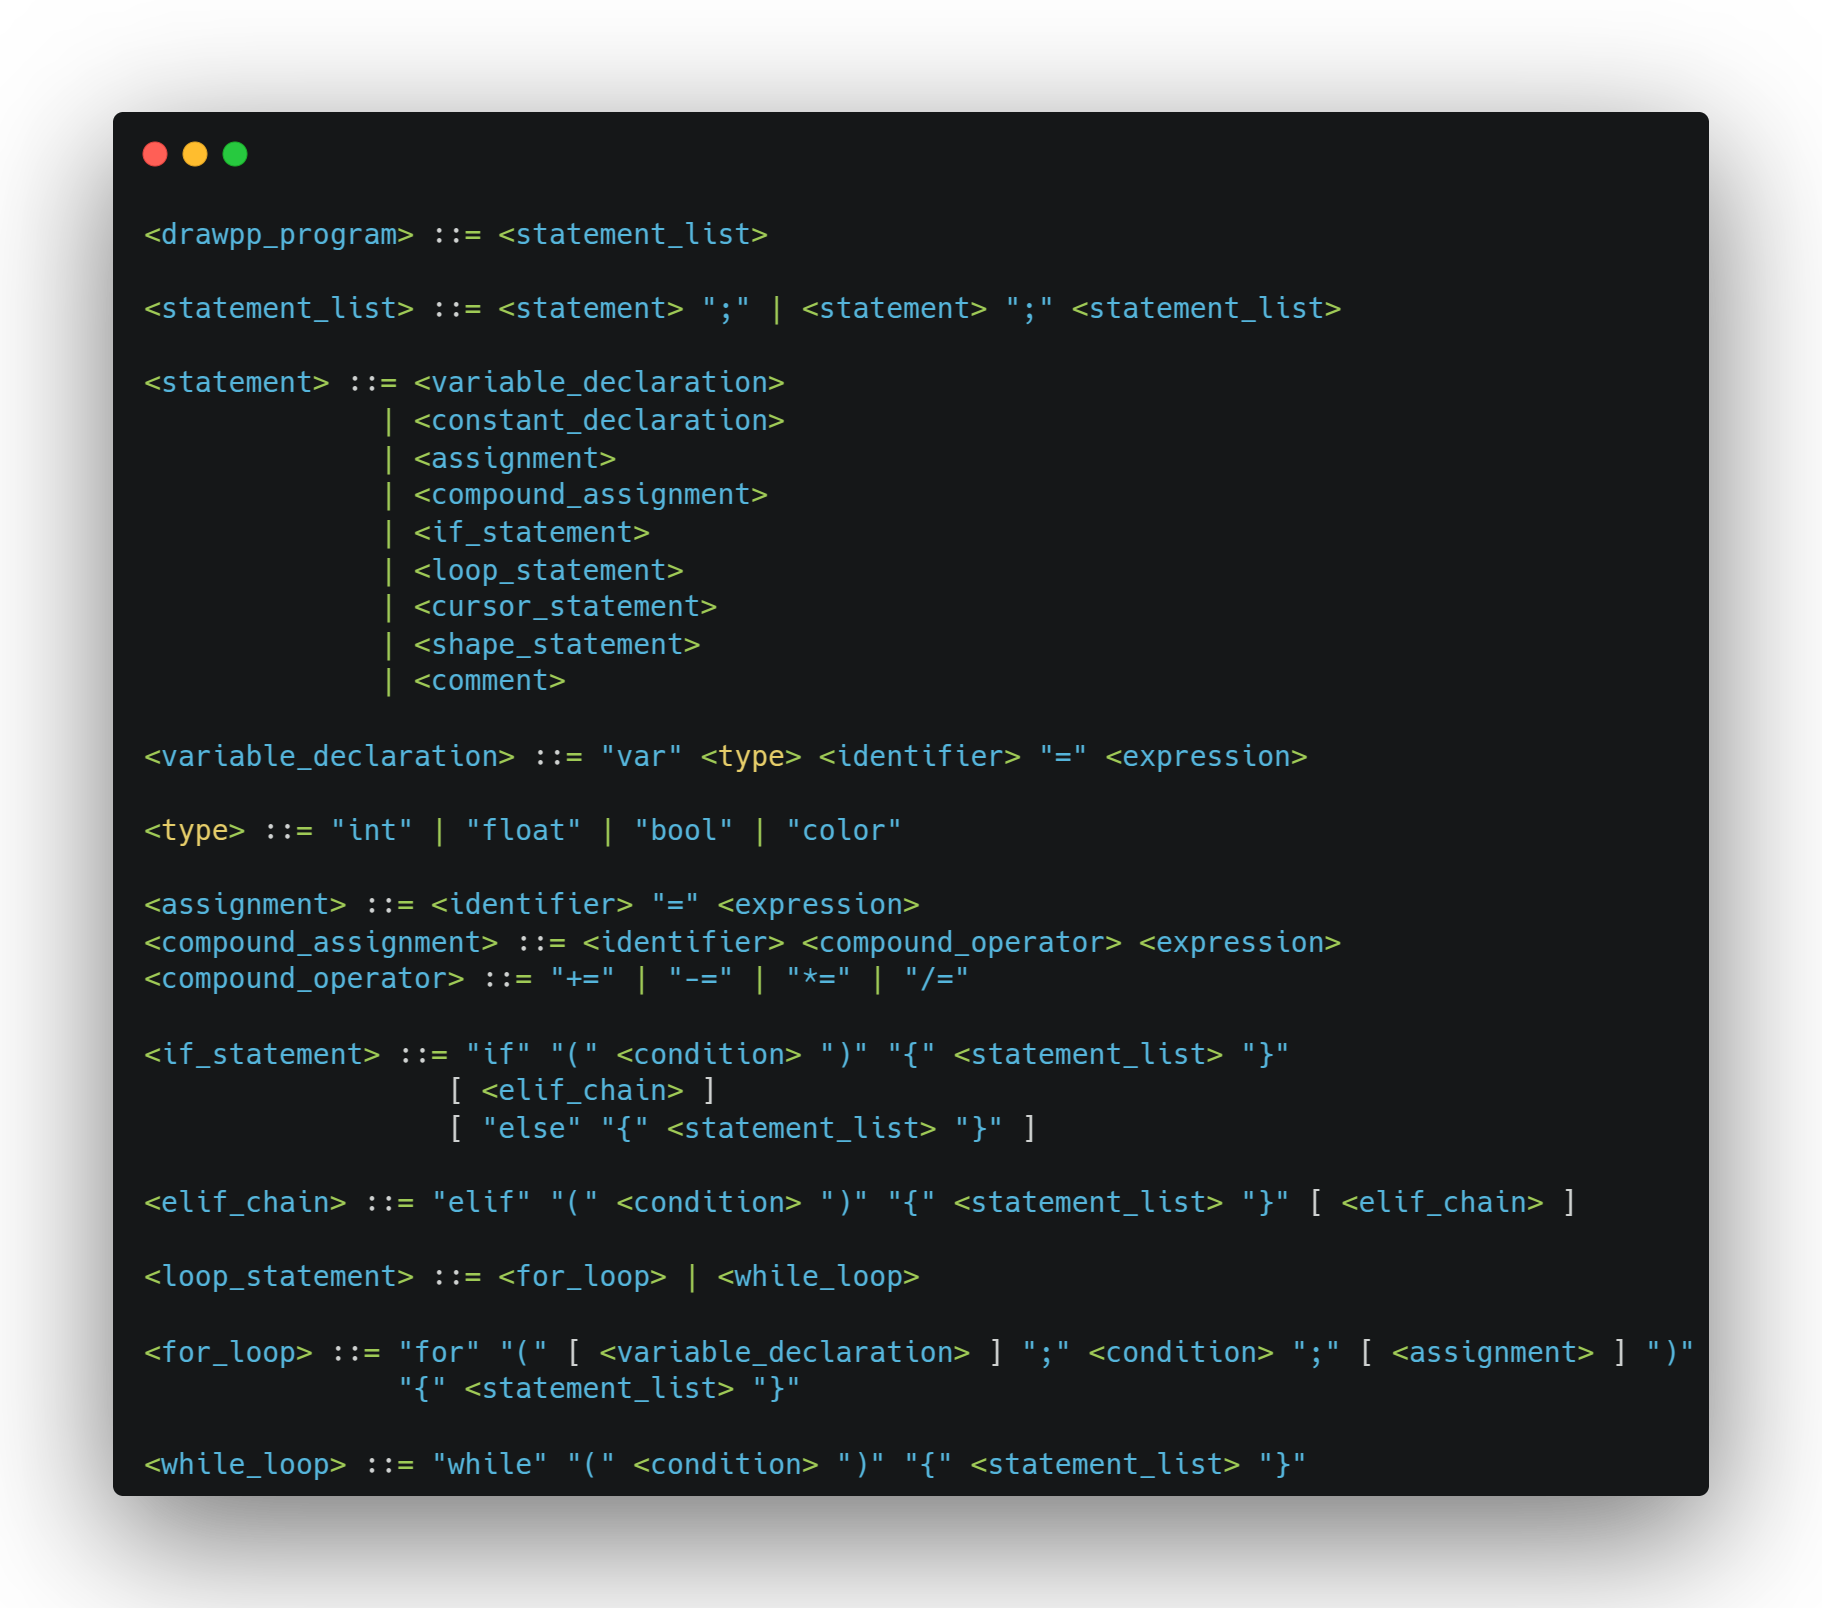
\includegraphics[width=0.9\linewidth]{assets/code/bnf1.png}
\end{figure}
\begin{figure}[H]
    \centering
    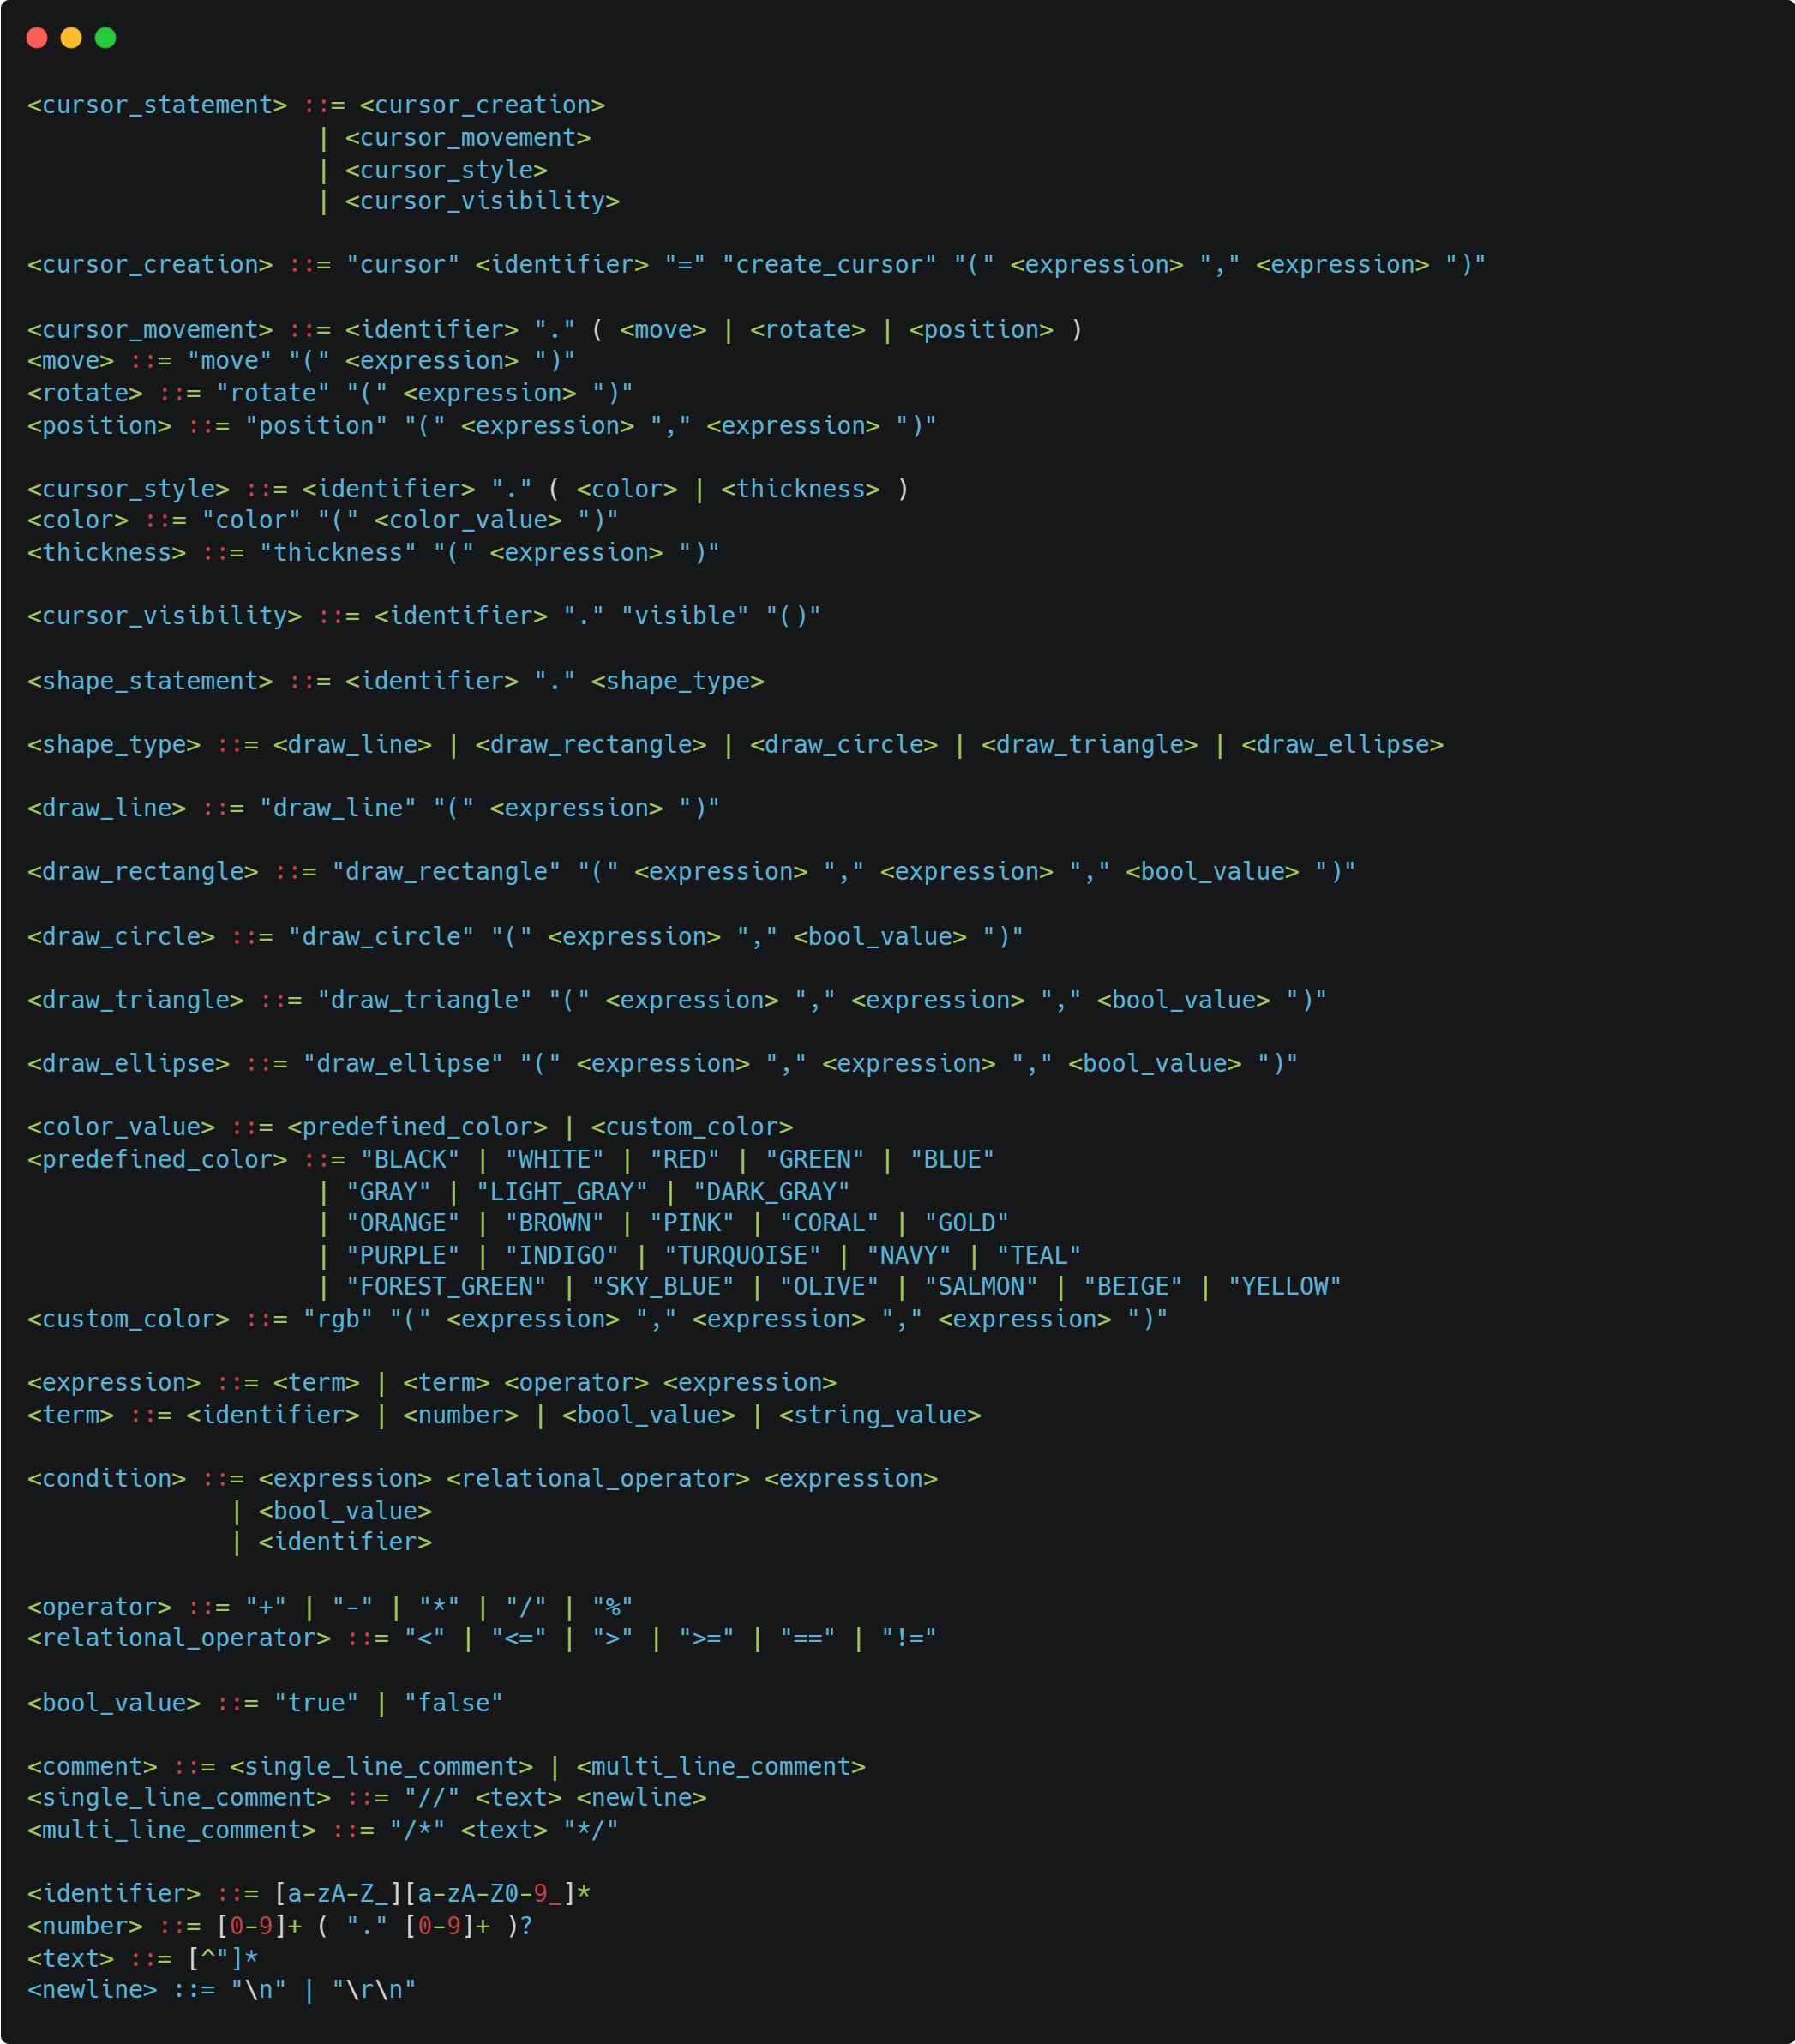
\includegraphics[width=1\linewidth]{assets/code/bnf2-3.png}
\end{figure}



\section{Variables Obligatoires}
Pour garantir un fonctionnement correct, chaque programme Draw++ doit definir les dimensions de la fenêtre graphique au debut. Ces dimensions sont specifiees par deux variables obligatoires :
\begin{itemize}
    \item \texttt{windowWidth} : Definit la largeur de la fenêtre.
    \item \texttt{windowHeight} : Definit la hauteur de la fenêtre.
\end{itemize}
Voici un exemple de declaration correcte :
\begin{lstlisting}[language=Draw++]
var int windowWidth = 500;
var int windowHeight = 500;
\end{lstlisting}
Ces declarations doivent apparaître avant toute autre instruction. Toute omission entraînera une erreur à l'execution.

\section{elements de Base}

\subsection{Terminaison des Instructions}
Chaque instruction doit se terminer par un point-virgule (\texttt{;}) afin de separer les instructions.
\begin{lstlisting}[language=Draw++]
var int x = 10;  // Declaration d'une variable
cursor.move(100);  // Deplacement du curseur
\end{lstlisting}

\subsection{Commentaires}
Les commentaires sont ignores à l'execution et permettent de documenter le code :
\begin{itemize}
    \item \textbf{Commentaires sur une ligne} : Utilisez \texttt{//}.
    \item \textbf{Commentaires multi-lignes} : Utilisez \texttt{/* ... */}.
\end{itemize}
\begin{lstlisting}[language=Draw++]
// Ceci est un commentaire sur une ligne
/* Ceci est un commentaire
   multi-lignes */
\end{lstlisting}

\subsection{Delimiteurs}
Les delimiteurs structurent le code et incluent :
\begin{itemize}
    \item \texttt{\{\}} : Pour delimiter les blocs d'instructions.
    \item \texttt{()} : Pour entourer les arguments des fonctions.
\end{itemize}

\section{Types et Variables}

\subsection{Declaration des Variables}
Les variables sont declarees avec le mot-cle \texttt{var}, suivi de leur type, de leur nom et de leur valeur initiale.
\begin{figure}[H]
    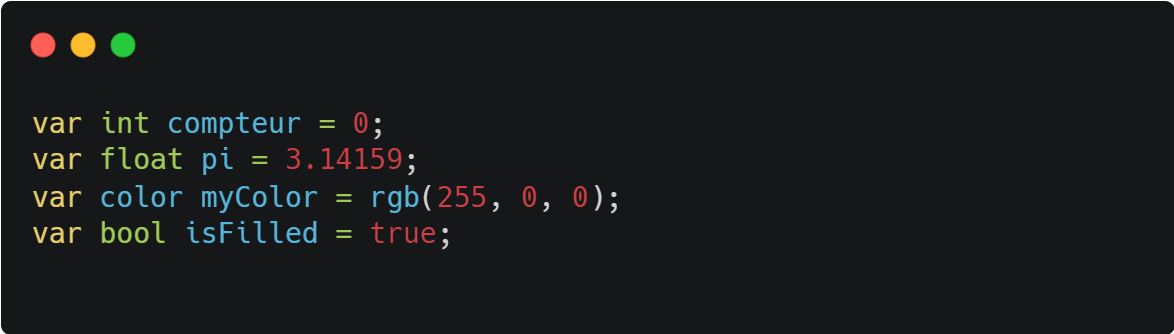
\includegraphics[width=1\linewidth]{assets/code/variables.png}
\end{figure}


\section{Structures de Contrôle}

\subsection{Conditions}
Les structures conditionnelles permettent d'executer des blocs de code selon des conditions :
\begin{itemize}
    \item \begin{verbatim} if (<condition>) { <bloc d'instructions> }\end{verbatim}
    \item \begin{verbatim} elif (<condition>) { <bloc d'instructions> }\end{verbatim}
    \item \begin{verbatim} else { <bloc d'instructions> }\end{verbatim}
    \begin{figure}[H]
    \centering
    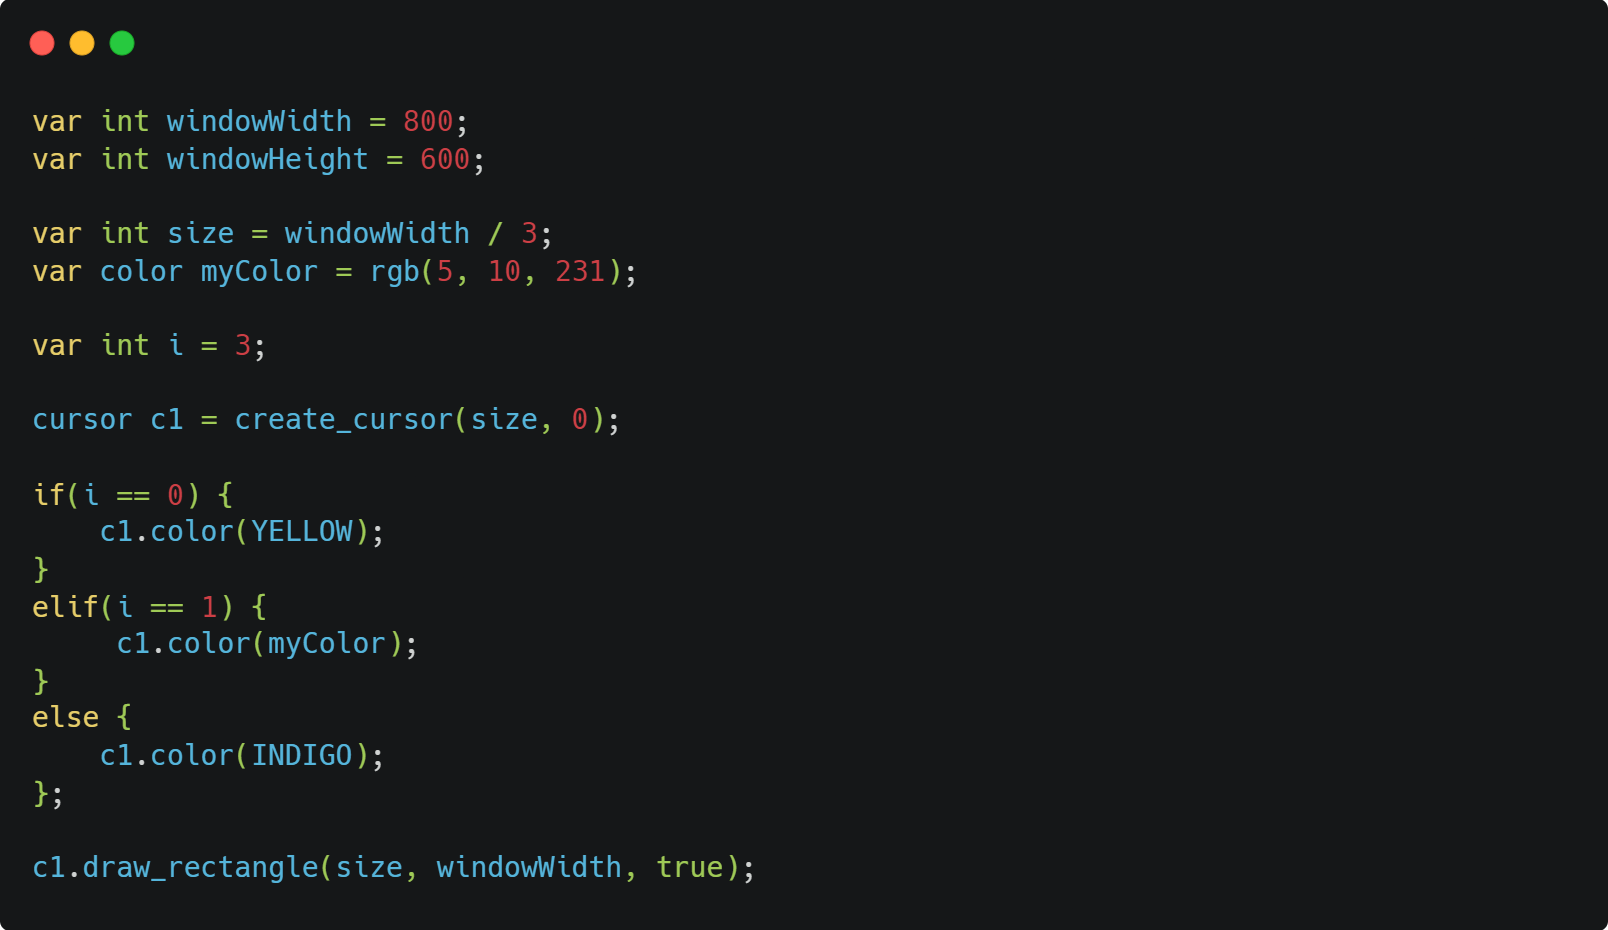
\includegraphics[width=1\linewidth]{assets/code/if_dpp.png}
    \caption{\centering Exemple de code conditionnel dans Draw++, montrant l'utilisation de la structure if-elif-else pour determiner la couleur d'un rectangle selon une condition.}
\end{figure}
\begin{figure}[H]
    \centering
    
\includegraphics[width=0.5\linewidth]{assets/render/if.png}
    \caption{\centering Rendu graphique correspondant à l'execution du code conditionnel, illustrant le changement de couleur du rectangle.}
\end{figure}
\end{itemize}

\subsection{Boucles}
Draw++ prend en charge deux types de boucles principales :
\begin{itemize}
    \item \begin{verbatim} while (<condition>) { <bloc d'instructions> } \end{verbatim}

    \begin{figure}[H]
    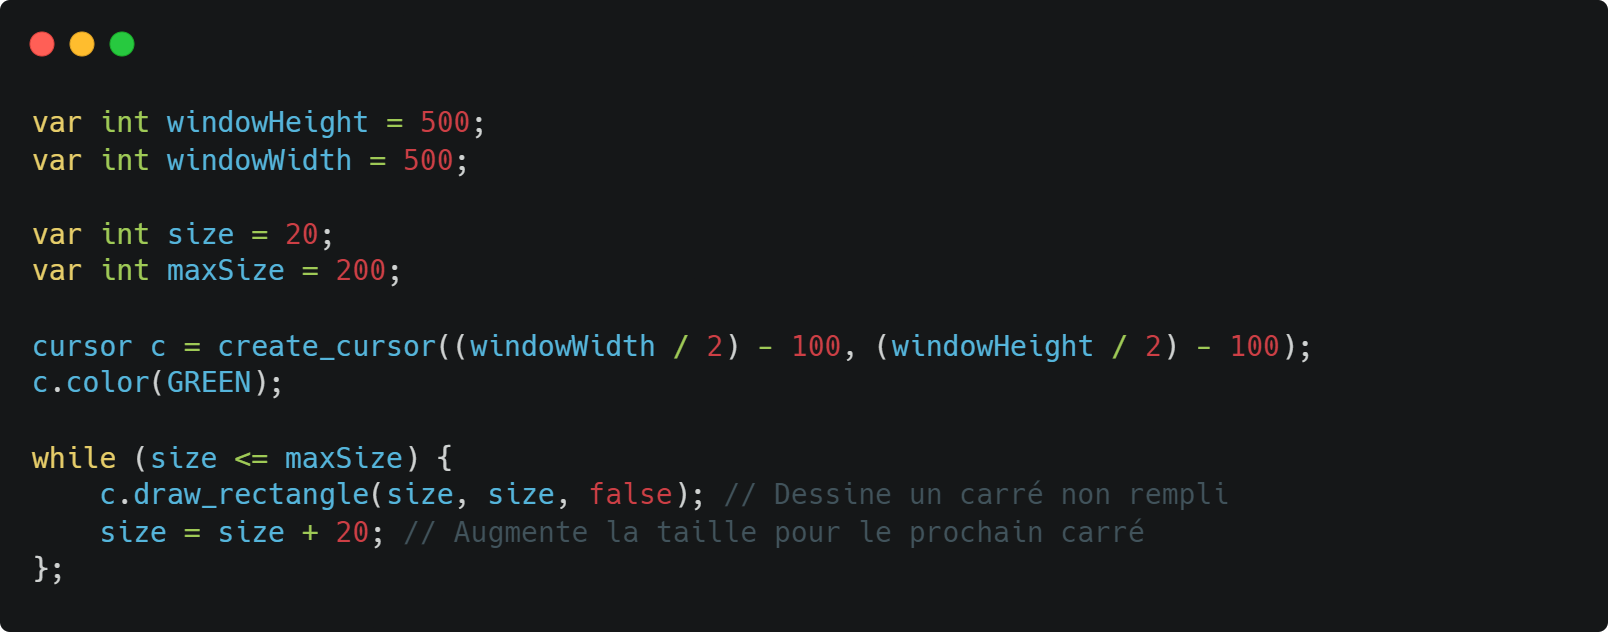
\includegraphics[width=1\linewidth]{assets/code/While_dpp.png}
    \caption{\centering Exemple d'utilisation de la boucle while pour dessiner des carres imbriques.}
\end{figure}
\begin{figure}[H]
    \centering
    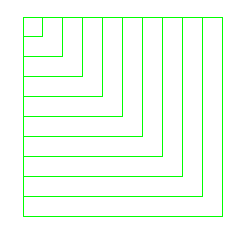
\includegraphics[width=0.3\linewidth]{assets/render/while.png}
    \caption{\centering Rendu graphique montrant le resultat de la boucle while, illustrant des carres imbriques dans un carre plus grand.}
\end{figure}

    \item \begin{verbatim}for (<initialisation>; <condition>; <mise à jour>){
<bloc d'instructions>}\end{verbatim}
    \begin{figure}[H]
    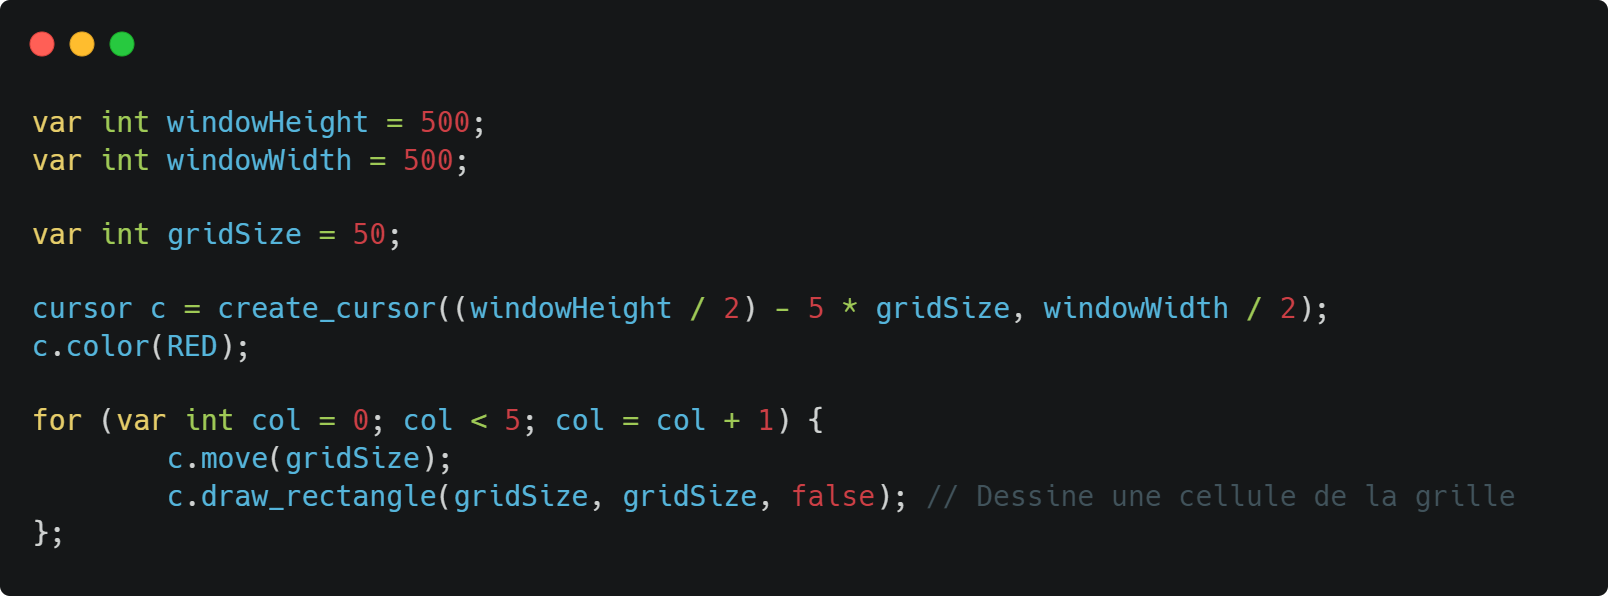
\includegraphics[width=1\linewidth]{assets/code/for1_dpp.png}
    \caption{\centering Exemple d'utilisation de la boucle for pour dessiner une serie de carres.}
\end{figure}
\begin{figure}[H]
    \centering
    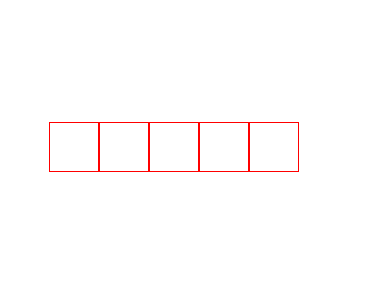
\includegraphics[width=0.4\linewidth]{assets/render/for.png}
    \caption{\centering Rendu graphique illustrant la liste de carres dessines à l'aide de la boucle for.}
\end{figure}
\begin{figure}[H]
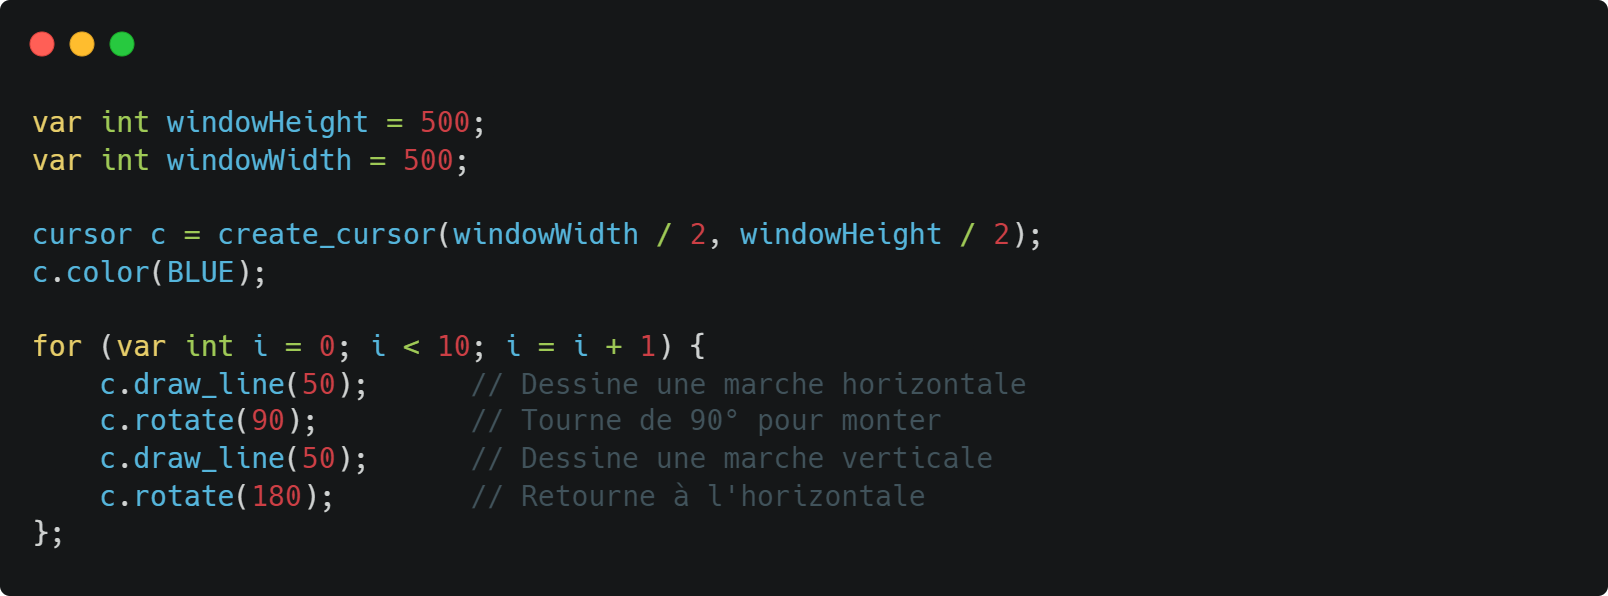
\includegraphics[width=1\linewidth]{assets/code/for2_dpp.png}
\caption{\centering Exemple d'utilisation de la boucle for pour dessiner une croix, où chaque iteration contribue à former les lignes de la croix}
\end{figure}
\begin{figure}[H]
    \centering
    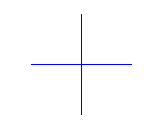
\includegraphics[width=0.3\linewidth]{assets/render/for2.png}
    \caption{\centering Rendu graphique montrant la croix creee par la boucle for, avec deux lignes perpendiculaires dessinees au centre.}
\end{figure}

\end{itemize}

\section{Manipulation du Curseur}
Le curseur est l'objet central pour dessiner. Il est defini avec la syntaxe suivante :
\begin{lstlisting}[language=Draw++]
cursor <identifiant> = create_cursor(<x>, <y>);
\end{lstlisting}
Les proprietes et methodes principales du curseur incluent :
\begin{itemize}
    \item \texttt{cursor.move(distance)} : Deplace le curseur.
    \item \texttt{cursor.rotate(angle)} : Tourne le curseur.
    \item \texttt{cursor.color(<couleur>)} : Definit la couleur.
    \item \texttt{cursor.thickness(<valeur>)} : Definit l'epaisseur du trait.
    \item \texttt{cursor.visible()} : Contrôle la visibilite du curseur.
\end{itemize}

\newpage
Exemple de creation et utilisation du curseur :
\begin{lstlisting}[language=Draw++]
cursor c = create_cursor(0, 0);
c.color(RED);
c.move(50);
\end{lstlisting}

\section{Dessiner des Formes}
Les formes peuvent être dessinees avec les methodes du curseur :
\begin{itemize}
    \item \texttt{cursor.draw\_line(longueur)} : Dessine une ligne.
    \item \texttt{cursor.draw\_rectangle(largeur, hauteur, rempli)} : Dessine un rectangle.
    \item \texttt{cursor.draw\_circle(rayon, rempli)} : Dessine un cercle.
    \item \texttt{cursor.draw\_triangle(base, hauteur, rempli)} : Dessine un triangle.
    \item \texttt{cursor.draw\_ellipse(largeur, hauteur, rempli)} : Dessine une ellipse.
\end{itemize}
Exemples :
\begin{lstlisting}[language=Draw++]
// Dessiner une ligne
cursor c = create_cursor(0, 0);
c.draw_line(100);

// Dessiner un rectangle rempli
c.draw_rectangle(50, 100, true);

// Dessiner un cercle non rempli
c.draw_circle(30, false);
\end{lstlisting}

\section{Couleurs et Styles}
Le curseur peut être personnalise avec des couleurs predefinies ou des couleurs personnalisees. Exemple :
\begin{lstlisting}[language=Draw++]
c.color(RED);
c.thickness(3);  // Definit l'epaisseur du trait
c.color(rgb(255, 0, 0));  // Rouge personnalise
\end{lstlisting}



\chapter{Description du traducteur}

\section{Architecture du traducteur}
Le traducteur de Draw++ est un système qui convertit le code source ecrit dans le langage Draw++ en code C intermediaire, prêt à être compile. Ce processus de traduction s'effectue en plusieurs etapes cles, chacune ayant pour but de transformer le code dans un format plus proche de l'execution.

\begin{enumerate}
    \item \textbf{Analyse lexicale} : Dans cette phase, le code source est decompose en tokens, qui sont les plus petites unites syntaxiques. Par exemple, des mots-cles comme \texttt{cursor}, \texttt{var}, \texttt{if}, ainsi que les identifiants et les operateurs, sont extraits du code source.
    \item \textbf{Analyse syntaxique} : Une fois que les tokens ont ete generes, le traducteur construit un arbre syntaxique abstrait (AST). Cet arbre represente la structure logique du programme, où chaque nœud correspond à une construction du langage (par exemple, une expression, une condition, ou une affectation).
    \item \textbf{Analyse semantique} : À ce stade, le traducteur verifie la validite des types, la coherence des variables, et l'integrite du programme. Cette etape s'assure que les operations sont effectuees sur des types compatibles (par exemple, eviter de tenter d'ajouter un entier à une chaîne de caractères).
    \item \textbf{Generation de code} : Enfin, le traducteur genère le code C intermediaire, qui est une version optimisee et executable de l'AST. Ce code est ensuite prêt à être compile par un compilateur C classique.
\end{enumerate}

\section{Processus de traduction}
Prenons un exemple simple pour illustrer le processus de traduction, où un programme ecrit en Draw++ est traduit en C intermediaire.

\subsection{Code Draw++}
Le code suivant est ecrit en Draw++ pour creer un curseur et dessiner un rectangle (qui peut egalement être utilise pour representer un carre si les côtes sont egaux) :

\begin{lstlisting}[language=Draw++]
cursor c = create_cursor(0, 0);
c.draw_rectangle(50, 50, false);
\end{lstlisting}

Le programme commence par declarer un curseur \texttt{c} en appelant la fonction \texttt{create\_cursor} avec les coordonnees (0, 0). Ensuite, la methode \texttt{draw\_rectangle} est utilisee pour dessiner un rectangle de 50 unites de largeur et 50 unites de hauteur. Le paramètre \texttt{false} indique que le rectangle ne doit pas être rempli.

\subsection{Code C genere}
Le traducteur convertit ce code Draw++ en code C, qui pourrait ressembler à ce qui suit :

\begin{lstlisting}[language=Draw++]
// Creation du curseur
Cursor* c = createCursor(0.0, 0.0);

// Dessin du rectangle (non rempli)
drawRectangle(c, 50.0, 50.0, false);
\end{lstlisting}

Dans cette etape de la traduction :
\begin{itemize}
    \item La fonction \texttt{create\_cursor(0, 0)} en Draw++ est traduite en \texttt{createCursor(0.0, 0.0)} en C. Les coordonnees sont converties en types \texttt{float} pour maintenir la coherence avec la representation C des positions en coordonnees flottantes.
    \item La methode \texttt{c.draw\_rectangle(50, 50, false)} devient un appel de fonction \texttt{drawRectangle(c, 50.0, 50.0, false)} en C. Le curseur \texttt{c} est passe comme un pointeur (\texttt{Cursor*}), et les dimensions du rectangle sont converties en \texttt{float} pour correspondre à la signature de la fonction generee.
\end{itemize}

\chapter{Bibliothèque graphique Draw++ (DPP)}

\section{Introduction à Draw++}
Draw++ (DPP) est une bibliothèque graphique conçue pour offrir une interface intuitive et performante pour le dessin graphique. Construit sur la base de SDL2, DPP enrichit les fonctionnalites de cette dernière en integrant des abstractions et outils adaptes à la manipulation graphique. Cette bibliothèque vise à reduire la complexite de l’utilisation directe de SDL2 tout en permettant une creativite sans limite.

\section{Fonctionnalites principales de Draw++}
La bibliothèque Draw++ offre des fonctionnalites avancees pour simplifier et enrichir le processus de creation graphique. Voici une presentation detaillee de ses principales capacites.

\subsection{Gestion des Curseurs}
Le concept central de DPP repose sur l’utilisation des curseurs. Ces entites permettent de simplifier le positionnement et la gestion graphique.

\begin{itemize}
    \item \textbf{Creation de curseurs} : Creez plusieurs curseurs avec \texttt{create\_cursor()} pour une manipulation flexible.
    \item \textbf{Operations intuitives} : Deplacement \texttt{move\_cursor()}, rotation \texttt{rotate\_cursor()}, et contrôle de la visibilite.
    \item \textbf{Personnalisation} : Changez la couleur (\texttt{set\_cursor\_color}) et l’epaisseur des traces (\texttt{set\_cursor\_thickness}).
\end{itemize}

\paragraph{Exemple :}
\begin{lstlisting}[language=C]
Cursor* c = create_cursor(100, 100); // Creation d'un curseur
set_cursor_color(c, red);            // Couleur rouge
move_cursor(c, 50);                 // Deplacement de 50 pixels
rotate_cursor(c, 90);               // Rotation de 90 degres
cursor_draw_line(c, 100);           // Dessin d'une ligne
\end{lstlisting}

\subsection{Dessin de Formes Geometriques}
Draw++ permet de dessiner des formes geometriques en simplifiant les calculs complexes.

\begin{itemize}
    \item \textbf{Lignes} : Tracez des lignes avec \texttt{cursor\_draw\_line()}.
    \item \textbf{Rectangles et cercles} : Gerez les dimensions et remplissages avec \texttt{cursor\_draw\_rectangle()} et \texttt{cursor\_draw\_circle()}.
    \item \textbf{Ellipses et triangles} : Creez des formes avancees avec \texttt{cursor\_draw\_ellipse()} et \texttt{cursor\_draw\_triangle()}.
\end{itemize}

\paragraph{Exemple :}
\begin{lstlisting}[language=C]
Cursor* c = create_cursor(200, 150);

// Dessiner un rectangle rempli
cursor_draw_rectangle(c, 200, 100, true);

// Dessiner un cercle non rempli
cursor_draw_circle(c, 50, false);

// Dessiner une ellipse
cursor_draw_ellipse(c, 120, 80, true);

// Dessiner un triangle
cursor_draw_triangle(c, 100, 50, false);
\end{lstlisting}

\subsection{Gestion des Couleurs}
La gestion des couleurs est intuitive avec DPP.

\begin{itemize}
    \item \textbf{Couleurs predefinies} : Utilisez \texttt{red}, \texttt{green}, \texttt{blue}, etc.
    \item \textbf{Couleurs personnalisees} : Creez des couleurs avec \texttt{custom\_color()}.
    \item \textbf{Attributs dynamiques} : Modifiez facilement les couleurs et styles des formes dessinees.
\end{itemize}

\paragraph{Exemple :}
\begin{lstlisting}[language=C]
// Creer une couleur personnalisee
SDL_Color myColor = custom_color(128, 0, 128, 255); // Violet opaque

// Appliquer la couleur au curseur
set_cursor_color(c, myColor);
\end{lstlisting}

\section{Avantages de Draw++}
Draw++ se distingue par plusieurs atouts majeurs :

\begin{itemize}
    \item \textbf{Facilite d'utilisation} : Une interface claire pour acceder aux outils graphiques sans complexite.
    \item \textbf{Flexibilite} : Une conception modulaire permettant d'ajouter facilement des fonctionnalites.
    \item \textbf{Support et documentation} : Une documentation complète et des exemples pour guider les developpeurs.
\end{itemize}

\section{Conclusion}
Draw++ offre une solution puissante et intuitive pour la programmation graphique, reduisant la complexite de SDL2 tout en apportant des outils specialises et adaptes à divers projets. Que ce soit pour un usage educatif ou professionnel, DPP simplifie le developpement tout en augmentant la creativite des utilisateurs.





\chapter{Gestion des erreurs}

La gestion des erreurs dans Draw++ repose sur une architecture modulaire qui couvre l'integralite du pipeline de compilation : lexicale, syntaxique et semantique. Chaque etape identifie des erreurs specifiques et propose des solutions adaptees pour aider l'utilisateur à corriger son code rapidement et efficacement.

\section{Types d'erreurs et traitements associes}

\begin{itemize}
    \item \textbf{Erreurs lexicales :} Detectees lors de la conversion du code en tokens.
    \begin{itemize}
        \item \textit{Caractères invalides :} Presence de symboles non reconnus dans le langage.
        \begin{itemize}
            \item \textbf{Traitement :} Proposer de supprimer ou remplacer les caractères non valides.
        \end{itemize}
        \item \textit{Chaînes non terminees :} Oubli d'un guillemet fermant.
        \begin{itemize}
            \item \textbf{Traitement :} Suggerer d'ajouter le guillemet manquant (\texttt{"}).\\
        \end{itemize}
    \end{itemize}

    \item \textbf{Erreurs syntaxiques :} Surviennent lors de l'analyse de la structure logique du code.
    \begin{itemize}
        \item \textit{Jetons inattendus :} Utilisation incorrecte de symboles ou d'instructions (exemple : \texttt{)} non appariee).
        \begin{itemize}
            \item \textbf{Traitement :} Verifier les parenthèses, accolades et points-virgules.
        \end{itemize}
        \item \textit{Types ou constructions attendus :} Absence d'un type ou mot-cle attendu.
        \begin{itemize}
            \item \textbf{Traitement :} Proposer des exemples valides, comme \texttt{var int myVar = 0;}
        \end{itemize}
        \item \textit{Terminaison manquante :} Oubli d'un point-virgule à la fin d'une instruction.
        \begin{itemize}
            \item \textbf{Traitement :} Indiquer la ligne concernee et suggerer d'ajouter un \texttt{;}.\\
        \end{itemize}
    \end{itemize}

    \item \textbf{Erreurs semantiques :} Verifient la validite logique et le sens du code.
    \begin{itemize}
        \item \textit{Variables non declarees :} Utilisation d'une variable sans declaration prealable.
        \begin{itemize}
            \item \textbf{Traitement :} Fournir des exemples de declaration pour corriger l'erreur.
        \end{itemize}
        \item \textit{Conflits de type :} Tentative d'assigner des types incompatibles.
        \begin{itemize}
            \item \textbf{Traitement :} Suggerer de convertir les types ou d'utiliser des types compatibles.
        \end{itemize}
        \item \textit{Variables dejà declarees :} Reutilisation d'un identifiant existant.
        \begin{itemize}
            \item \textbf{Traitement :} Proposer un nouveau nom ou la suppression de la declaration redondante.
        \end{itemize}
        \item \textit{Utilisation incorrecte des curseurs :} Methode appelee sur un objet non initialise ou non valide.
        \begin{itemize}
            \item \textbf{Traitement :} Fournir un exemple d'initialisation correcte.\\
        \end{itemize}
    \end{itemize}

    \item \textbf{Erreurs specifiques aux curseurs :} Ces erreurs sont propres au fonctionnement graphique de Draw++.
    \begin{itemize}
        \item \textit{Methode invalide :} Appel d'une methode inexistante pour un curseur.
        \begin{itemize}
            \item \textbf{Traitement :} Lister les methodes valides comme \texttt{move(distance)} ou \texttt{rotate(angle)}.
        \end{itemize}
        \item \textit{Proprietes incompatibles :} Essayer d'utiliser une couleur ou une epaisseur invalide.
        \begin{itemize}
            \item \textbf{Traitement :} Fournir des exemples valides, comme \texttt{cursor.color(RED);}.
        \end{itemize}
    \end{itemize}
\end{itemize}

\section{Exemple d'integration}

Un exemple typique de correction automatique :
\begin{lstlisting}[language=draw++]
var int x = 10
cursor c = create_cursor(0, 0);
c.move(100);
\end{lstlisting}

Erreur detectee : \textit{"Expected TokenType.SEMICOLON at line 1"} \\
\textbf{Suggestions :}
\begin{itemize}
    \item Ajouter un point-virgule après \texttt{var int x = 10;}.
\end{itemize}

\chapter{Interface de Developpement Integre (IDE)}

\section{Vue d'ensemble}
L'IDE Draw++ propose un environnement de developpement complet specialement conçu pour le langage Draw++. L'interface se divise en trois zones principales :
\begin{itemize}
    \item Un editeur de code avec numerotation des lignes
    \item Une zone de previsualisation graphique
    \item Un terminal integre
\end{itemize}
\begin{figure}
    \centering
    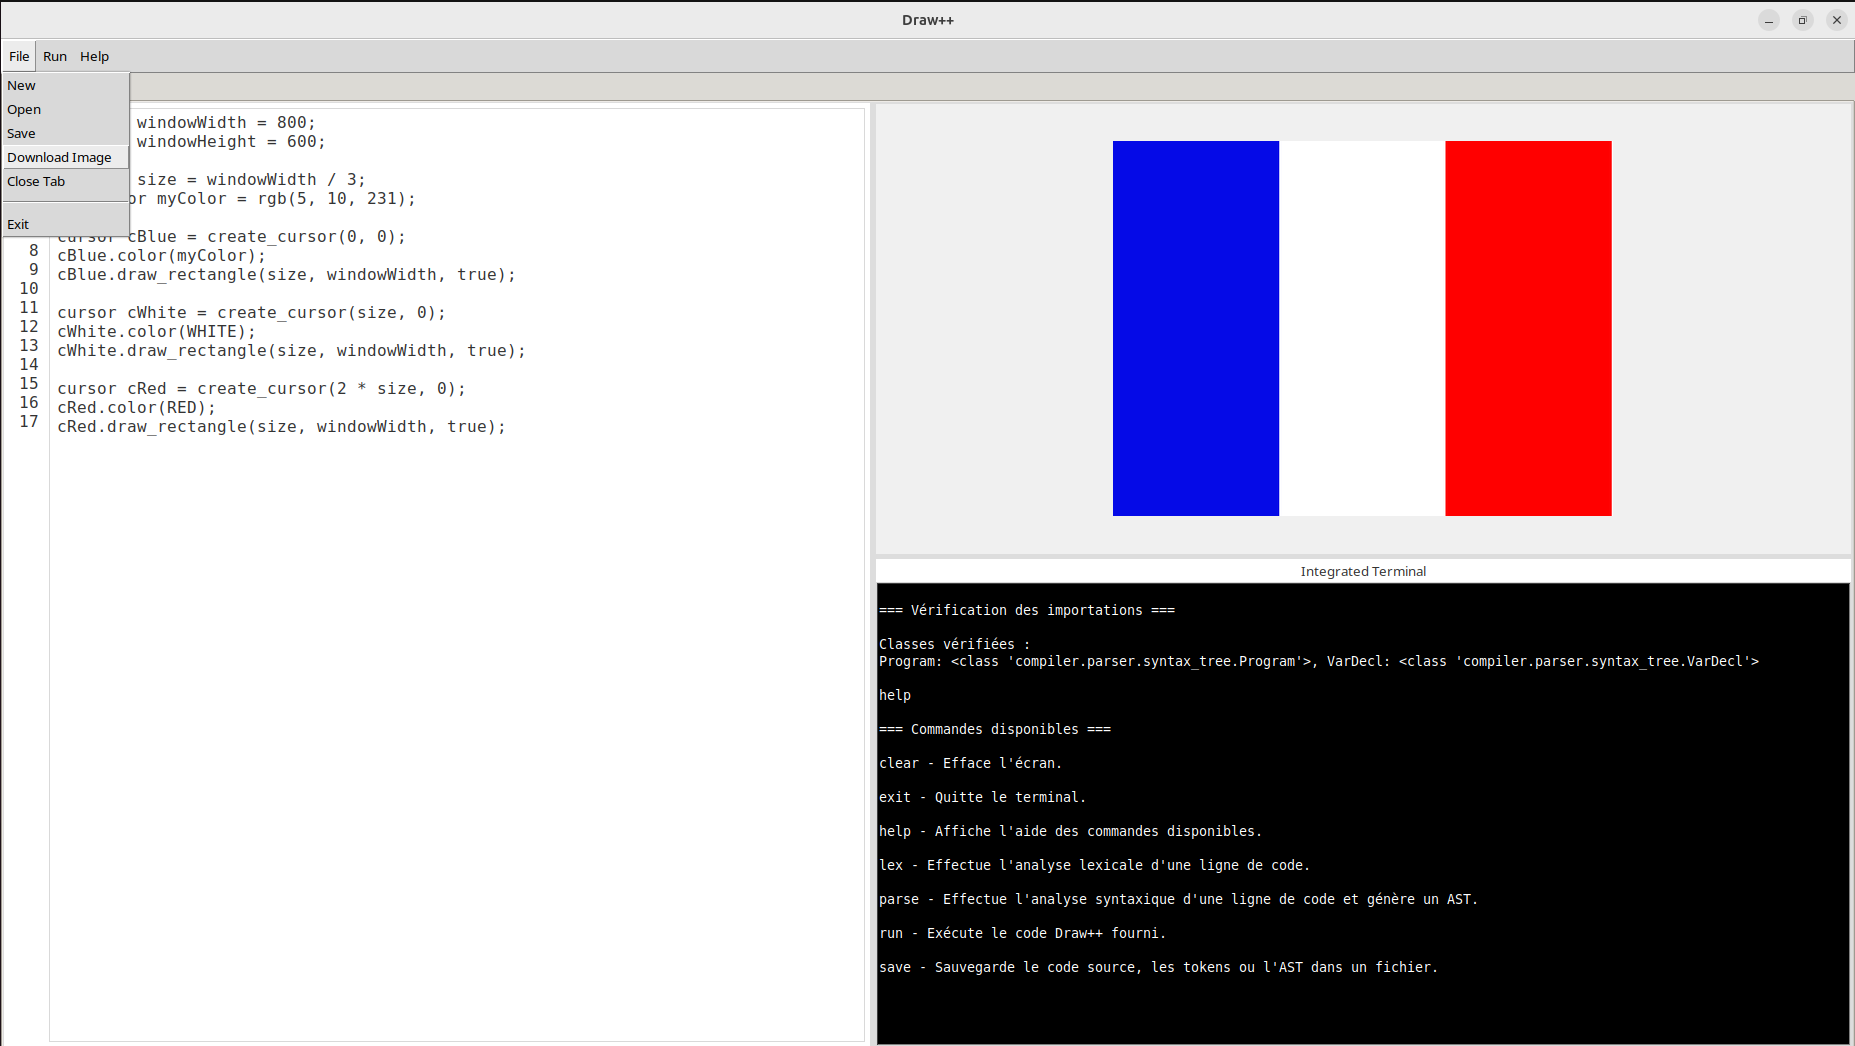
\includegraphics[width=0.9\linewidth]{assets/ide/image.png}
    \caption{Interface de Developpement Integre Draw++.}
    \label{fig:enter-label}
\end{figure}

\section{Composants principaux}

\subsection{Barre de menu}
La barre de menu en haut de l'interface offre plusieurs options essentielles :
\begin{itemize}
    \item \textbf{File} : Gestion des fichiers
    \begin{itemize}
        \item New : Creer un nouveau fichier
        \item Open : Ouvrir un fichier existant
        \item Save : Sauvegarder le fichier courant
        \item Download Image : Exporter le rendu graphique
        \item Close Tab : Fermer l'onglet actif
        \item Exit : Quitter l'application
    \end{itemize}
    \item \textbf{Run} : Execution du code
    \item \textbf{Help} : Accès à l'aide
\end{itemize}

\subsection{editeur de code}
L'editeur intègre plusieurs fonctionnalites avancees :
\begin{itemize}
    \item Numerotation automatique des lignes
    \item Coloration syntaxique pour le langage Draw++
    \item Mise en evidence des erreurs
    \item Support pour les commentaires (// et /* */)
\end{itemize}

\subsection{Zone de previsualisation}
La zone de previsualisation offre les caracteristiques suivantes :
\begin{itemize}
    \item Affichage du rendu graphique
    \item Mise à jour lors de l'execution du code
    \item Zone redimensionnable
    \item Aperçu fidèle des dimensions specifiees par \texttt{windowWidth} et \texttt{windowHeight}
\end{itemize}
\newpage
\subsection{Terminal integre}
Le terminal propose plusieurs commandes essentielles :
\begin{lstlisting}[style=customStyle]
clear  - Efface l'ecran
exit   - Quitte le terminal
help   - Affiche l'aide des commandes disponibles
lex    - Effectue l'analyse lexicale d'une ligne de code
parse  - Effectue l'analyse syntaxique et genere l'AST
run    - Execute le code Draw++
save   - Sauvegarde le code source, les tokens ou l'AST
\end{lstlisting}


\section{Fonctionnalites d'analyse et debogage}

\subsection{Analyse lexicale}
Le terminal affiche les informations detaillees pour chaque token genere :
\begin{itemize}
    \item Type du token
    \item Valeur
    \item Numero de ligne
    \item Position dans la ligne
\end{itemize}

Un exemple de sortie d'analyse lexicale :
\begin{figure}[H]
    \centering
    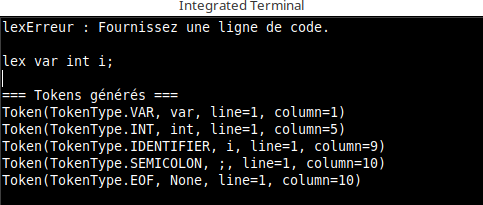
\includegraphics[width=0.7\linewidth]{assets/terminal/terminal.png}
    \label{fig:enter-label}
\end{figure}

\subsection{Retours d'erreur}
L'IDE fournit des messages d'erreur detailles pour differents types d'erreurs :
\begin{itemize}
    \item Erreurs de syntaxe
    \item Erreurs lexicales
    \item Erreurs semantiques
    \item Problèmes de compilation
\end{itemize}

\subsection{Verification en temps reel}
L'IDE effectue plusieurs verifications pendant la saisie :
\begin{itemize}
    \item Validation des variables obligatoires (\texttt{windowWidth}, \texttt{windowHeight})
    \item Verification de la syntaxe
    \item Detection des erreurs de type
    \item Validation des appels de methodes sur les curseurs
\end{itemize}

\section{Bonnes pratiques d'utilisation}

\subsection{Initialisation du projet}
Pour demarrer un nouveau projet efficacement :
\begin{itemize}
    \item Toujours commencer par definir \texttt{windowWidth} et \texttt{windowHeight}
    \item Organiser le code avec des commentaires descriptifs
    \item Sauvegarder regulièrement le travail
\end{itemize}

\subsection{Debogage}
Pour un debogage efficace :
\begin{itemize}
    \item Utiliser la commande \texttt{lex} pour verifier l'analyse lexicale
    \item Employer la commande \texttt{parse} pour valider la structure du code
    \item Consulter le terminal pour les messages d'erreur detailles
\end{itemize}


\chapter{Exemples d'execution}

Dans cette section, nous presentons plusieurs exemples d'execution utilisant le langage Draw++. Chaque exemple inclut le rendu graphique genere et la sortie du terminal.

\section{Exemple 1 : Dessin d'un cercle}
\begin{figure}[H]
    \centering
    
\includegraphics[width=0.45\textwidth]{assets/render/draw_circle.png}
    \caption{Rendu graphique du cercle.}
    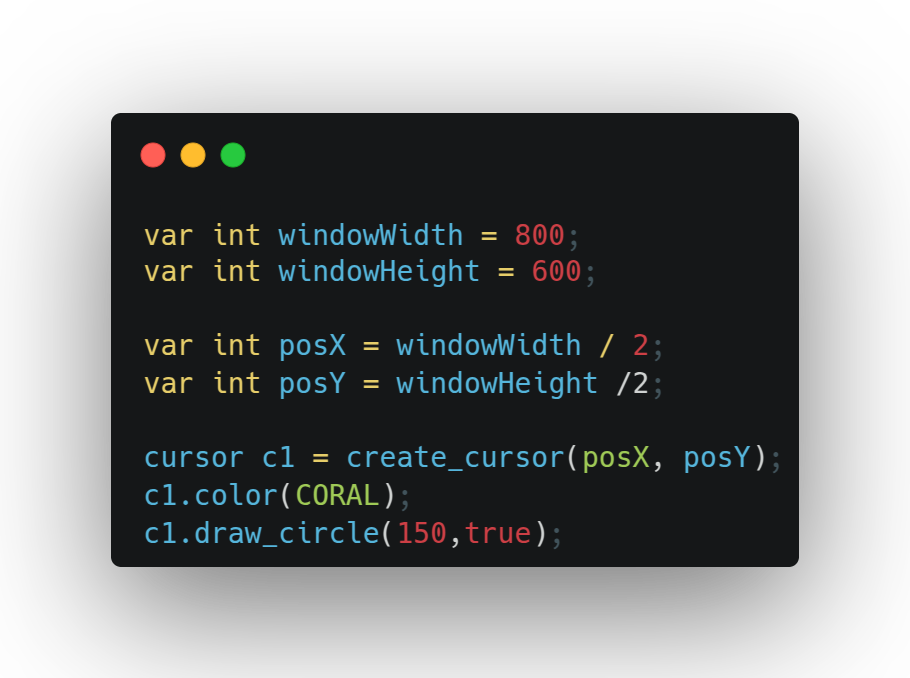
\includegraphics[width=0.9\textwidth]{assets/code/draw_circle_dpp.png}
    \caption{Code DPP pour dessiner un cercle.}
\end{figure}

\section{Exemple 2 : Dessin d'un triangle}
\begin{figure}[H]
    \centering
    
\includegraphics[width=0.45\textwidth]{assets/render/draw_triangle.png}
    \caption{Rendu graphique du triangle.}
    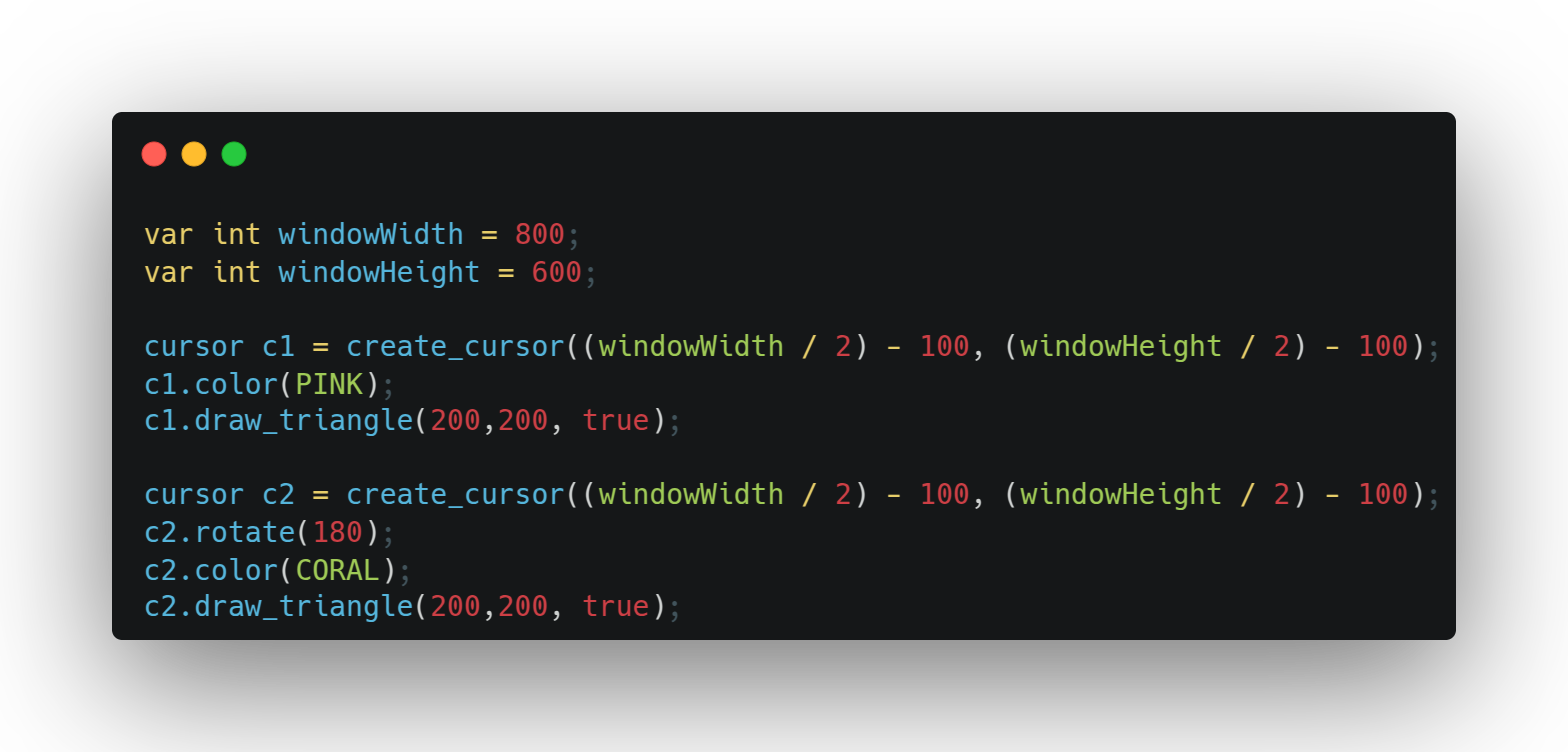
\includegraphics[width=0.9\textwidth]{assets/code/draw_triangle_dpp.png}
    \caption{Code DPP pour dessiner un triangle.}
\end{figure}

\section{Exemple 3 : Dessin du drapeau de la France}
\begin{figure}[H]
    \centering
    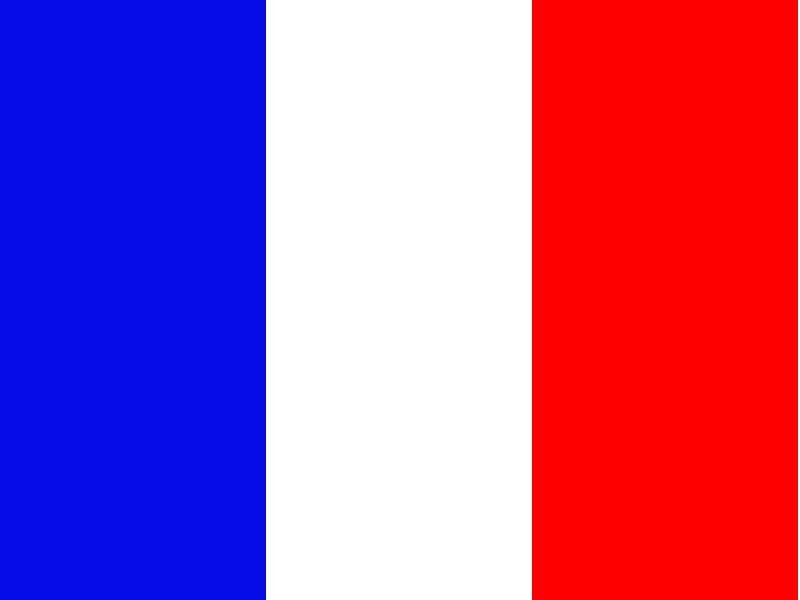
\includegraphics[width=0.45\textwidth]{assets/render/france.png}
    \caption{Rendu graphique du drapeau de la France.}
    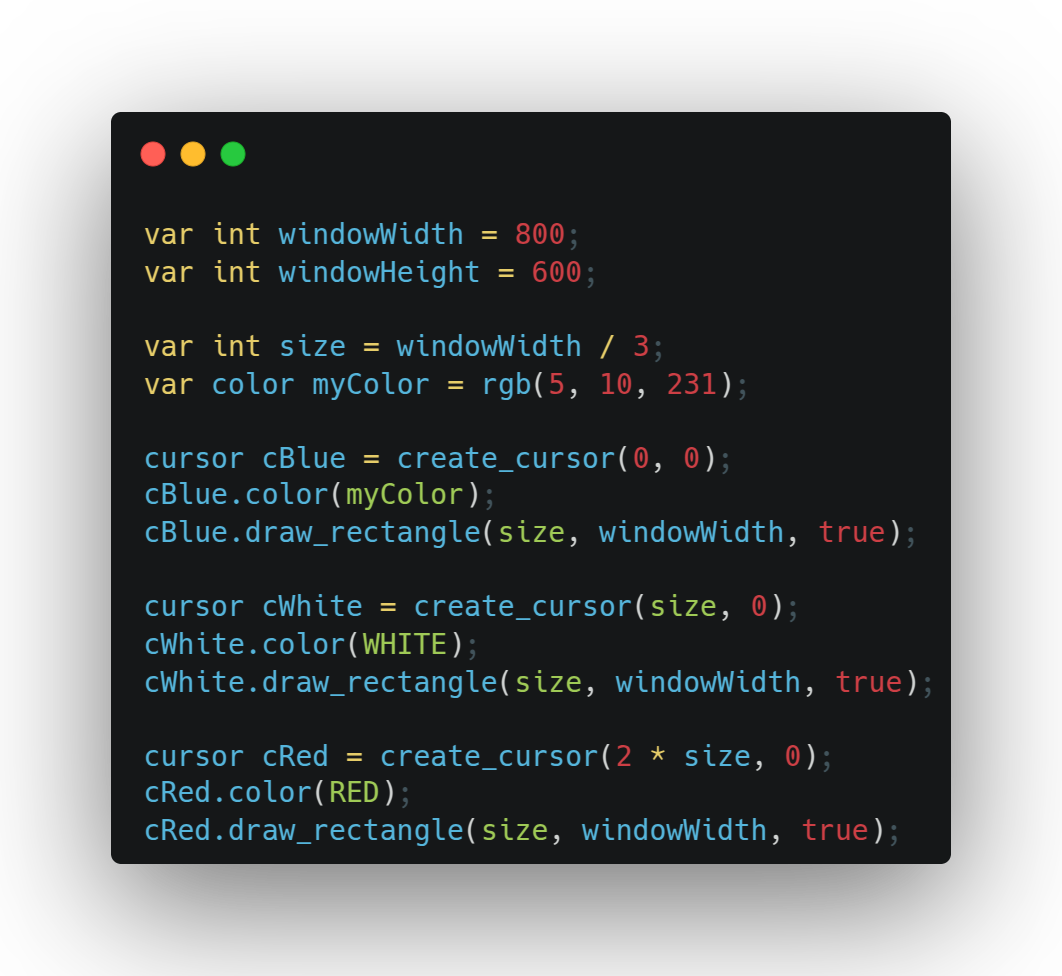
\includegraphics[width=0.8\textwidth]{assets/code/france_dpp}
    \caption{Code DPP pour dessiner le drapeau de la France.}
\end{figure}

\section{Exemple 4 : Dessin d'une ligne}
\begin{figure}[H]
    \centering
    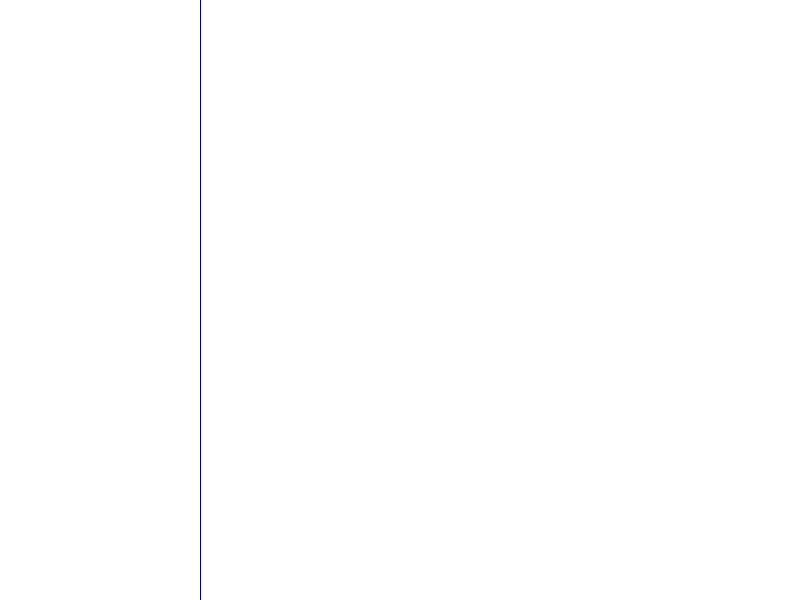
\includegraphics[width=0.45\textwidth]{assets/render/draw_line.png}
    \caption{Rendu graphique de la ligne.}
    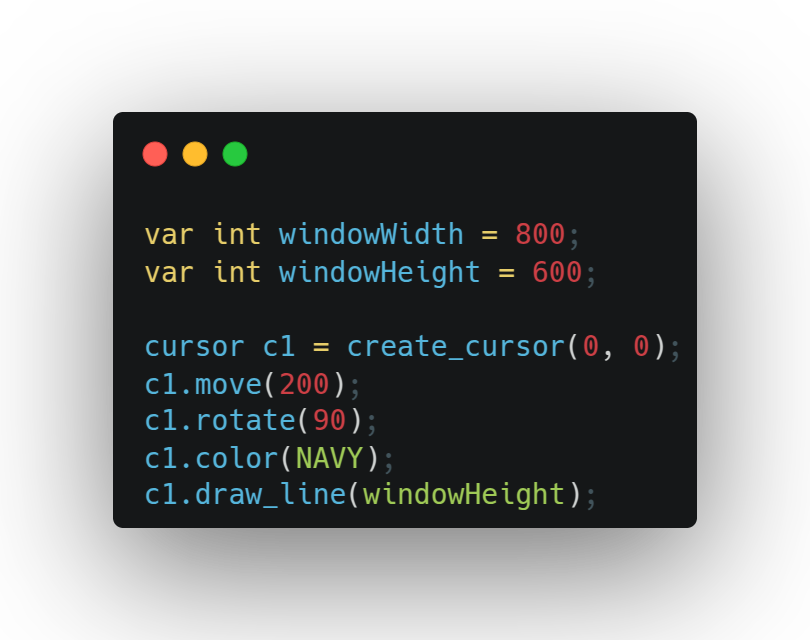
\includegraphics[width=0.8\textwidth]{assets/code/draw_line_dpp.png}
    \caption{Code DPP pour dessiner une ligne.}
\end{figure}

\section{Exemple 5 : Dessin d'un rectangle}
\begin{figure}[H]
    \centering
    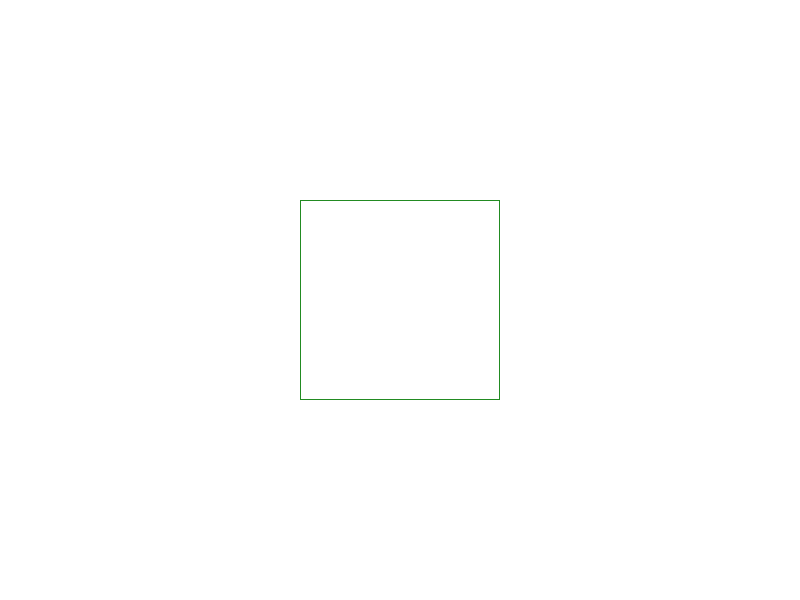
\includegraphics[width=0.7\textwidth]{assets/render/draw_rectangle.png}
    \caption{Rendu graphique du rectangle.}
    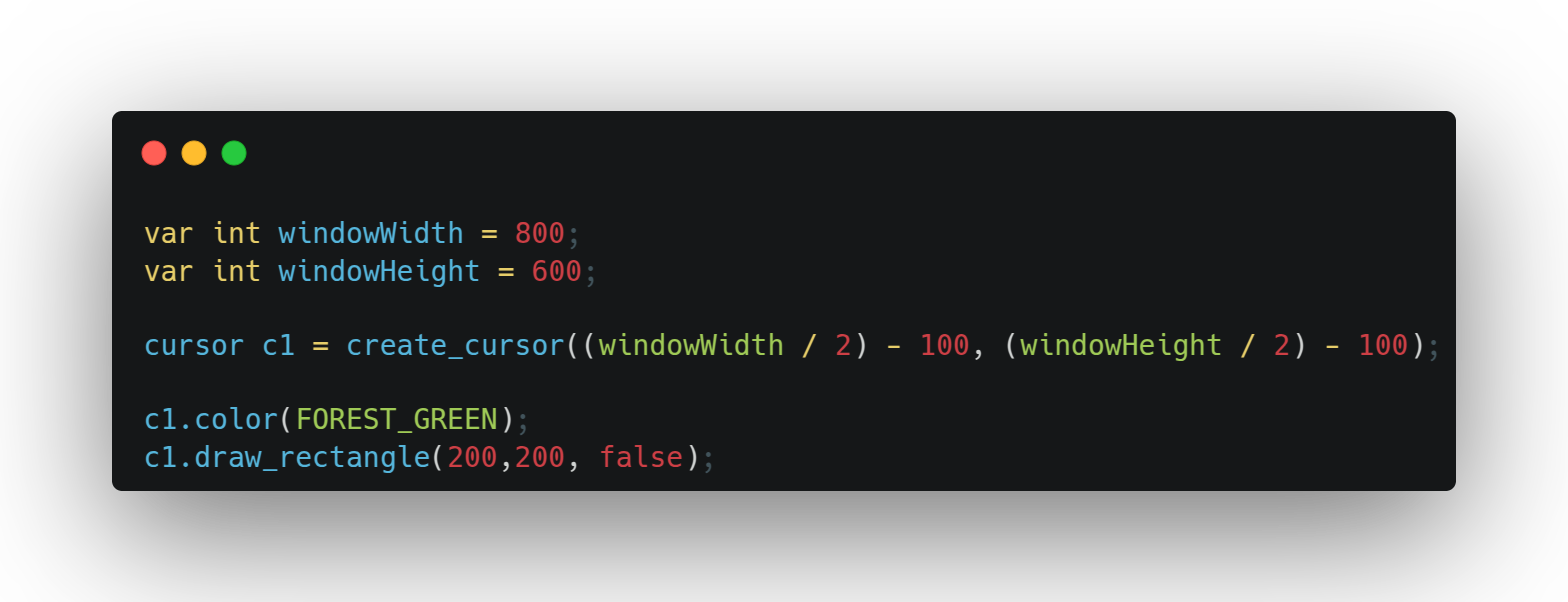
\includegraphics[width=1\textwidth]{assets/code/draw_rectangle_dpp.png}
    \caption{Code DPP pour dessiner un rectangle.}
\end{figure}

\section{Exemple 6 : Dessin d'une ellipse}
\begin{figure}[H]
    \centering
    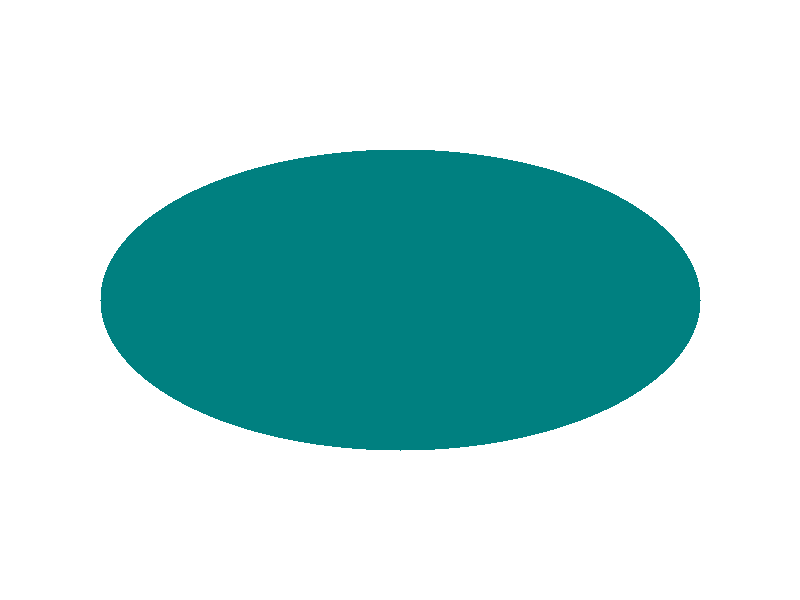
\includegraphics[width=0.45\textwidth]{assets/render/draw_ellipse.png}
    \caption{Rendu graphique de l'ellipse.}
    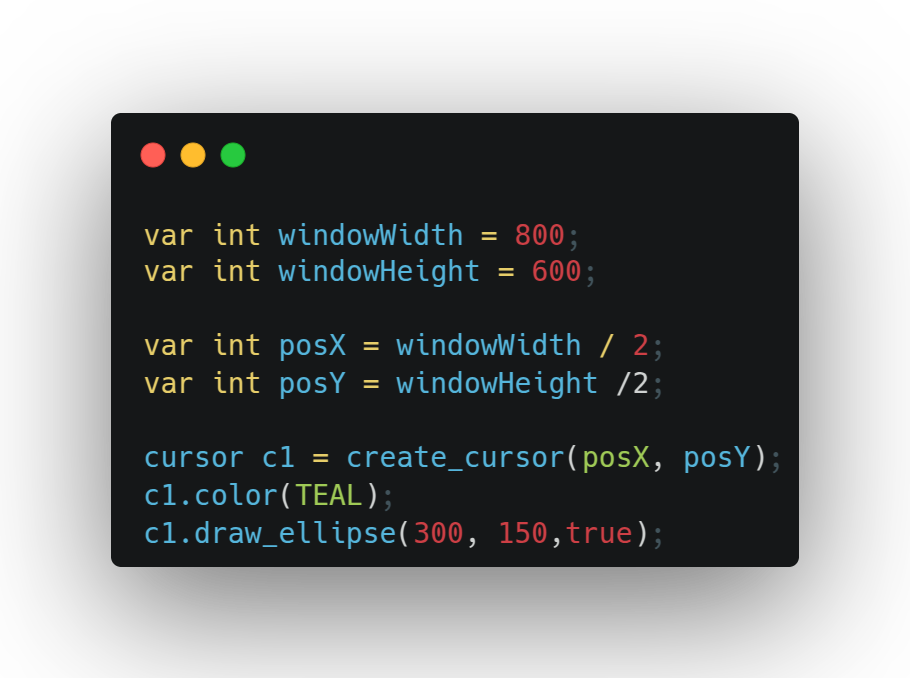
\includegraphics[width=0.8\textwidth]{assets/code/draw_ellipse_dpp.png}
    \caption{Code DPP pour dessiner une ellipse.}
\end{figure}

\newpage

\section{Sortie du terminal}
\begin{figure}[H]
    \centering
    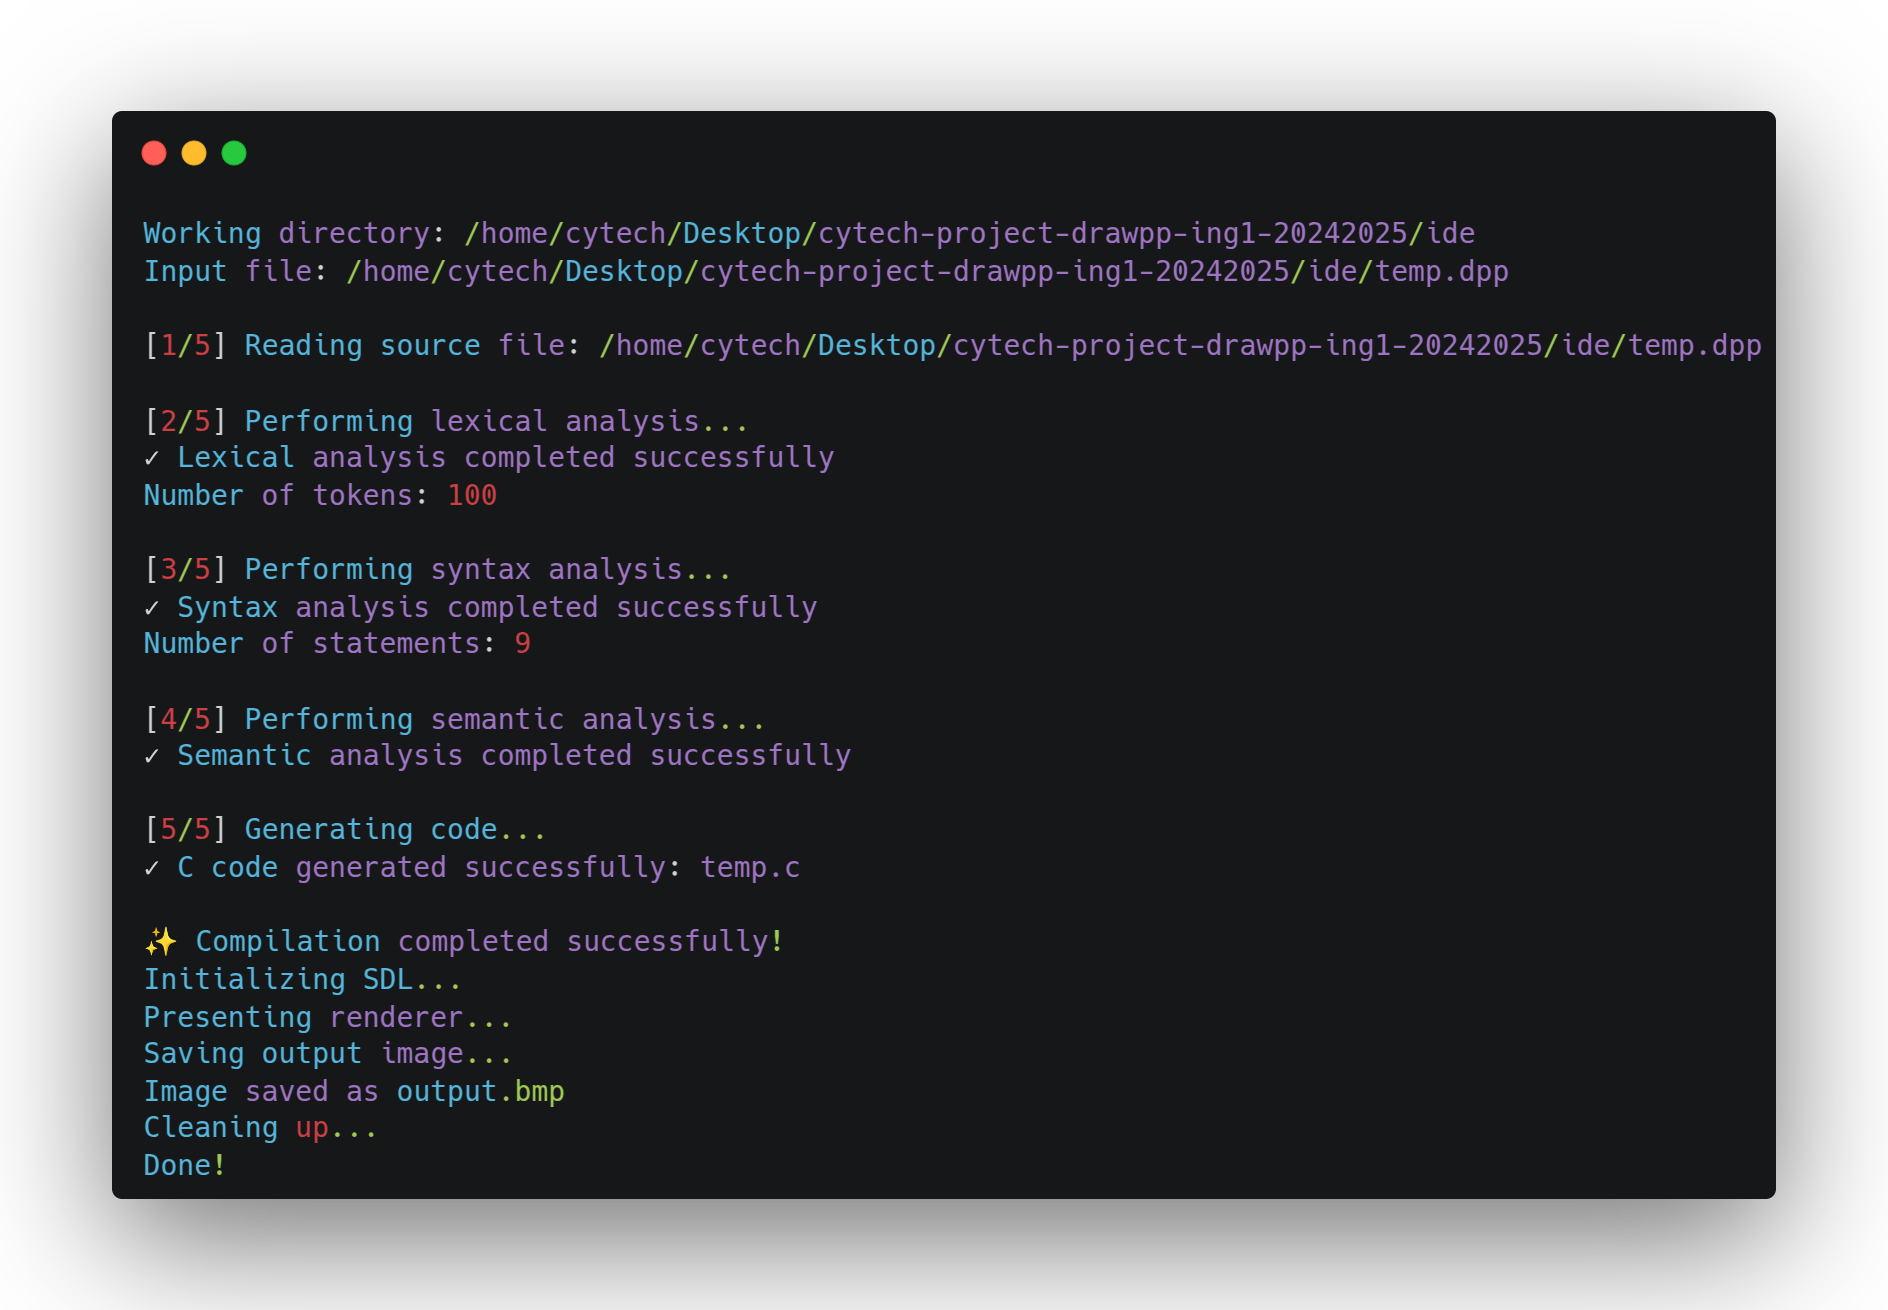
\includegraphics[width=1\textwidth]{assets/terminal/terminal_output_after_run.png}
\end{figure}

\newpage
\section{Autre exemple}
Voici un exemple complet avec l'utilisation d'une couleur personnalisée et l'utilsation d'autres fonctions de curseur. \textbf{cursor.visible()} qui permet de montrer le curseur sur l'image avec un petit carré. \textbf{cursor.thickness(<taille>)} qui permet d'augmenter l'épaisseur du trait.
\begin{figure}[H]
    \centering
    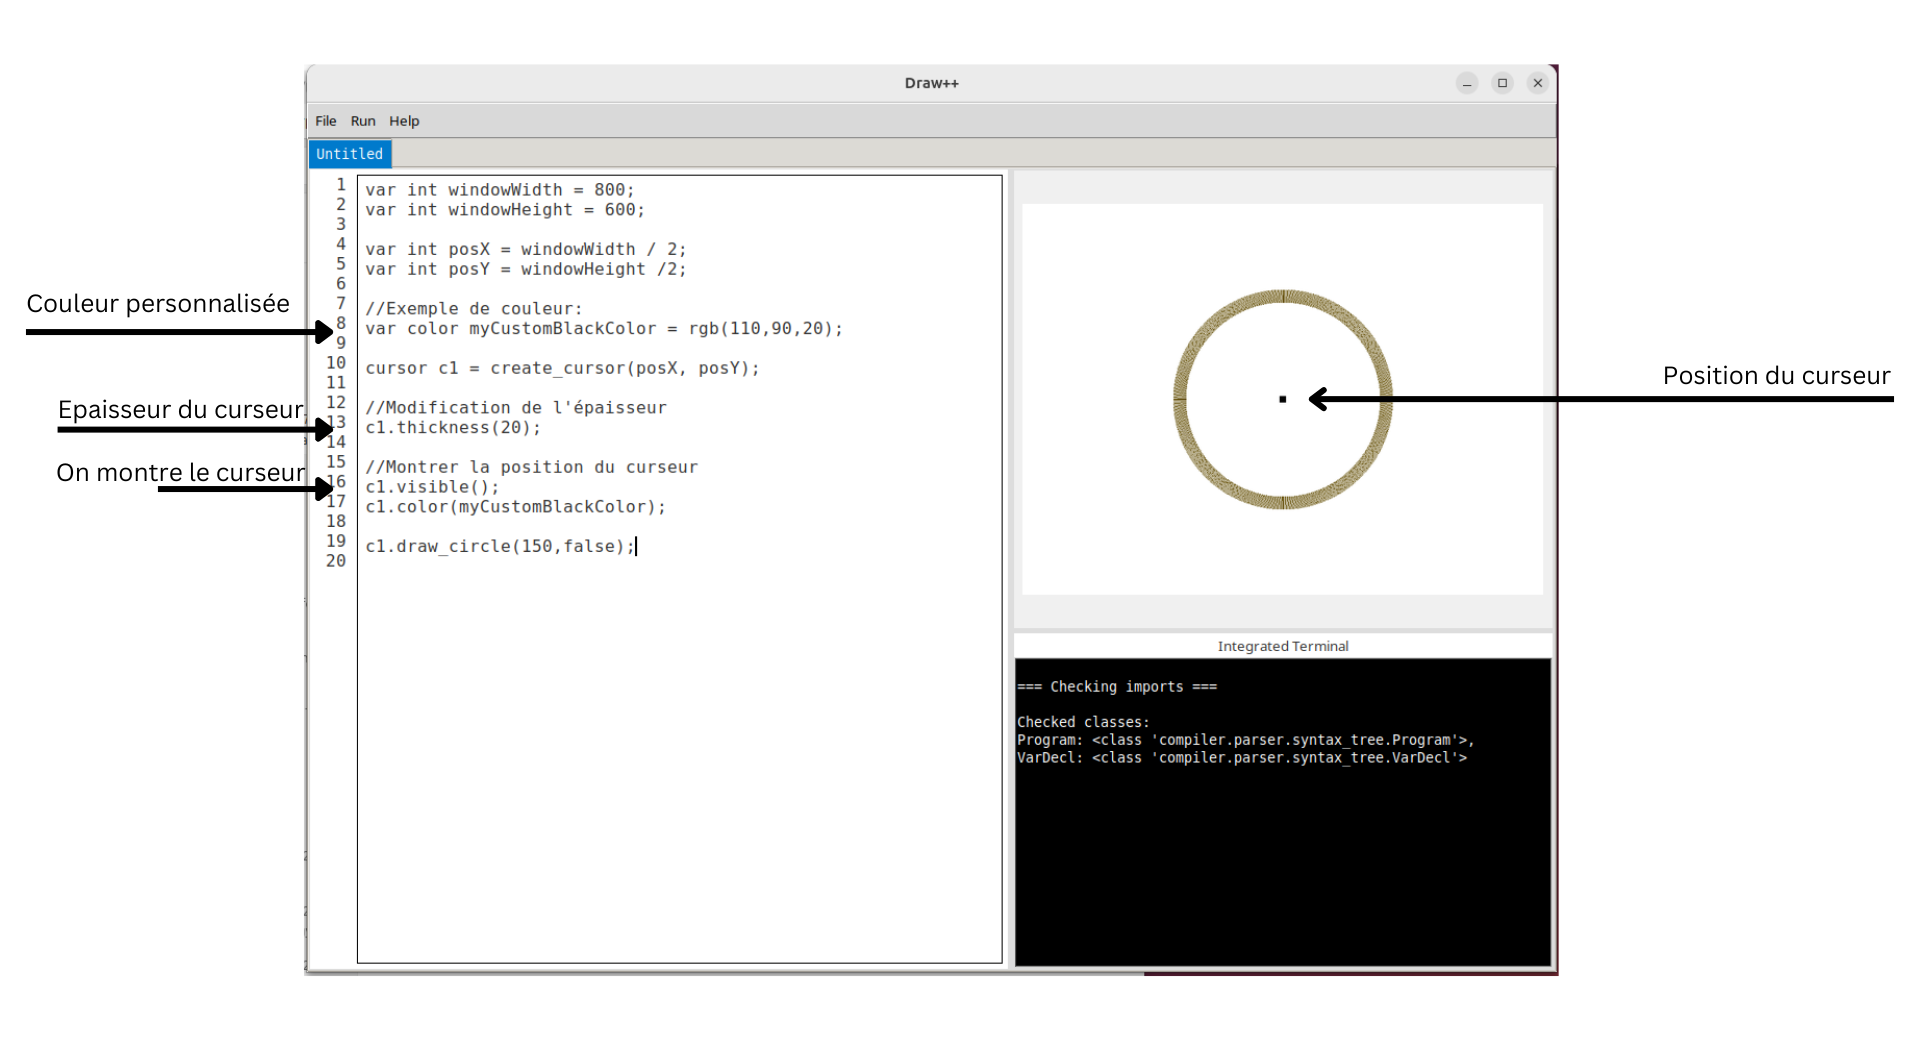
\includegraphics[width=1.2\textwidth]{assets/ide/image3.png}
\end{figure}

 \chapter{Conclusion}

Le projet Draw++ a permis la conception d'un langage graphique minimaliste, couple à un traducteur robuste, capable de transformer des instructions simples en formes visuelles. Le traducteur, conçu avec une attention particulière à la gestion des erreurs et à l’analyse syntaxique, garantit une execution fluide et precise du code. La structure du langage, combinee à des outils de manipulation des formes, offre une plateforme puissante pour explorer l'interaction entre programmation et visualisation graphique.

\end{document}